\documentclass[a4paper]{article}

% HEADER
\input{header_report.tex}

\setcounter{tocdepth}{2}

\begin{document}

% ==================================================================================================================================
% TITLEPAGE 

\begin{titlepage}
    \begin{center}
        %includegraphics[width=0.4\textwidth]{./images/logo_UT.png} \\[1cm]

        %
\includegraphics[height=2.5cm]{./images/logo_UT.png} 
        %\hspace{2cm}
        %
\includegraphics[height=2.5cm]{./images/logo_irit.png}
        %\\[1cm]

        \begin{tabular}{@{}c@{\hspace{2cm}}c@{}}
            
\includegraphics[height=2.5cm]{./images/logo_UT.png} & 
            
\includegraphics[height=3cm]{./images/logo_irit.png}
        \end{tabular}
        \\[1cm]

        {\Huge \textbf{Cross-disciplinary applications of the Toulbar2 solver}} \\[1cm]

        {\Large \textbf{UE : Introductory Research Project}} \\[2cm]

        \textbf{Authors :} \\[0.5cm]

        Hugo Garcia \\
        \href{mailto:hugo.garcia@univ-tlse3.fr}{hugo.garcia@univ-tlse3.fr}\\[0.5cm]

        Philippe Gauthier \\
        \href{mailto:philippe.gauthier@univ-tlse3.fr}{philippe.gauthier@univ-tlse3.fr}\\[0.5cm]

        Marco Sanfilippo \\
        \href{mailto:marco.sanfilippo@univ-tlse3.fr}{marco.sanfilippo@univ-tlse3.fr}\\[0.5cm]

        Mathis Francine-Habas \\
        \href{mailto:mathis.francine-habas@univ-tlse3.fr}{mathis.francine-habas@univ-tlse3.fr}\\[0.5cm]
        
        \vspace{0.3cm}
        \textbf{Supervisor :} \\[0.5cm]

        Martin Cooper \\
        (\small Lecturer and researcher at the Toulouse Institute of Computer Science Research - IRIT)
        \href{mailto:martin.cooper@univ-tlse3.fr}{martin.cooper@univ-tlse3.fr}\\[0.5cm]
        
        \vspace{0.5cm}
        \textbf{University :} University of Toulouse \\[0.1cm]
        \textbf{Adress :} 118 Narbonne road, 31062 Toulouse, France \\[0.5cm]
        \textbf{Date :} \today \\[2cm]

        \vfill
    \end{center}
\end{titlepage}

% ==================================================================================================================================
% ABSTRACT (RÉSUMÉ)

\newpage
\thispagestyle{plain}
\vspace*{\fill}

\begin{abstract}
    \centering
    \itshape
    \justify
    
    resumé à mettre ici
    
    \vspace{0.5cm}
    \noindent \textbf{Key Words :} Mathematics, Informatics, ..
\end{abstract}

\vspace*{\fill}

% ==================================================================================================================================
% TABLES ET LISTES

\newpage
% Table des matières
\tableofcontents

\newpage
% \begin{figure}...\caption{}...\end{figure})
\listoffigures

\newpage
% \begin{table}...\caption{}...\end{table})
\listoftables

\newpage
\section*{List of Acronyms}
\addcontentsline{toc}{section}{List of Acronyms}

% Le mot entre crochets [PLNE] sert à aligner le texte. 
% Mets ici l'acronyme le plus long de ta liste pour que l'espacement soit parfait.
\begin{acronym}[EDAC]
    \acro{WCSP}{Weighted Constraint Satisfaction Problem}
    \acro{CSP}{Constraint Satisfaction Problem}
    \acro{VCSP}{Valued Constraint Satisfaction Problem}
    \acro{CFN}{Cost Function Network}
    \acro{EPT}{Equivalence Preserving Transformations}
    \acro{SAC}{Soft Arc Consistency}
    \acro{FDAC}{Full Directional Arc Consistency}
    \acro{EDAC}{Existential Directional Arc Consistency}
    \acro{VAC}{Virtual Arc Consistency}
    \acro{OSAC}{Optimal Soft Arc Consistency}
    \acro{MILP}{Mixed-Integer Linear Programming}
    \acro{CP}{Constraint Programming}
    \acro{LP}{Linear Programming}
    \acro{MIP}{Mixed Integer Programming}
    \acro{MINLP}{Mixed Integer Non-Linear Programming}
    \acro{SBF}{Smart Brute-force}
\end{acronym}

\vspace{1cm}
\noindent\rule{\textwidth}{1pt}

% ==================================================================================================================================
% Introduction 

\newpage
\section*{Introduction}
%\addcontentsline{toc}{section}{Introduction}

exemple\cite{montalbano_multiple-choice_2022}


% ==================================================================================================================================
% PARTIE 1 : Algorithmic Foundations & Solver Development

\newpage
\section{Algorithmic Foundations \& Solver Development}

\subsection{An application to graph theory and the cluster editing problem}

texte



\subsection{Constraint programming for discrete integration in high dimensions}

texte


% ==================================================================================================================================
% PARTIE 2 : Proteine





% ==================================================================================================================================
% PARTIE 3 : Resource Management & Planning

\section{Resource Management \& Planning}

\subsection{Preamble}

Although the Toulbar2 solver has gained a strong reputation in the field of bioinformatics, 
the Cost Function Network formalism is proving particularly well-suited to classical operational research problems. 
The management and allocation of resources generally involve satisfying strict rules (hard constraints) 
whilst optimising quality criteria or preferences (soft constraints). 
This section illustrates how soft local consistency algorithms (such \ac{OSAC} \& \ac{EDAC}) implemented in Toulbar2 
enable the resolution of industrial-scale planning problems, whilst highlighting the strengths and limitations 
of these exact approaches compared to other paradigms such as \ac{MILP}.

\subsection{Spatio-temporal allocation and conflict management}


Planning and allocating physical resources often require merging two complex dimensions : space and time. 
This could mean rotating crops across agricultural land over several years. It could also involve coordinating 
flight paths in restricted airspace. These problems require satisfying strict rules while simultaneously optimizing quality criteria.

This subsection illustrates how the \ac{WCSP} formalism models these spatio-temporal environments. 
It also evaluates the efficiency of the Toulbar2 solver compared to other exact methods.
\newline

The crop allocation problem consists of assigning different crop types (the values) to agricultural plots (the variables) over a finite time horizon. 
The approach proposed by Akplogan et al. (2013)\cite{akplogan_solving_2013} stands out by simultaneously modeling spatial and temporal constraints at the farm level.
\newline

The model integrates two types of constraints:

\begin{itemize}
    \item \textbf{Hard constraints :} These guarantee agronomic feasibility. Examples include the minimum return time for a crop on the same plot, or respecting the biophysical properties of the soil.
    \item \textbf{Soft constraints :} These reflect the farmer's preferences. Examples include the spatio-temporal balance of the crops, or the beneficial effects of previous crops on the soil.
\end{itemize}

\begin{figure}[H]
    \centering
    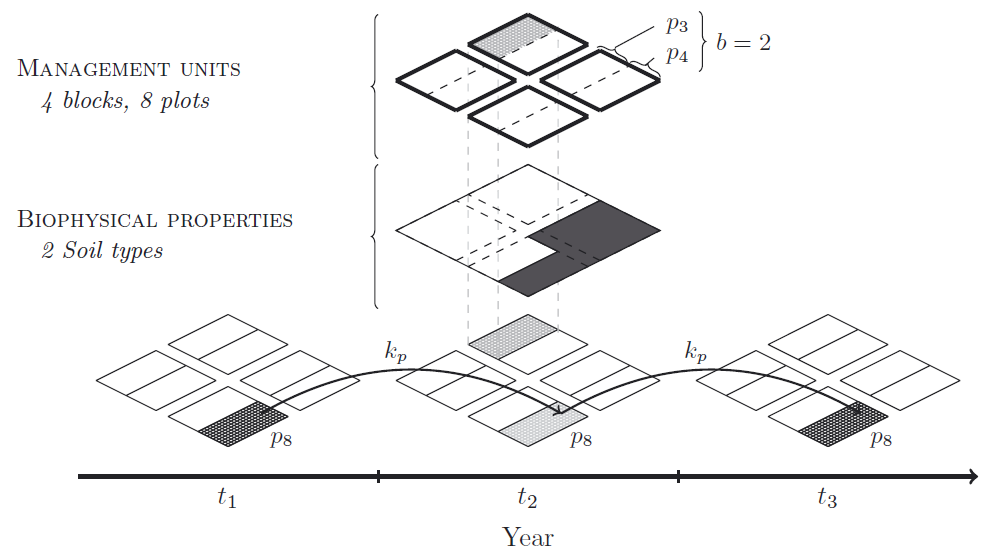
\includegraphics[width=\textwidth]{images/crop_allocation_explication.png}
    \caption{Schematic representation of the spatial and temporal aspects of the decision–making problem ($t_i$ : year, $b$ : block, $p_j$ : plot, $k_p$ : preceding effect)\cite{akplogan_solving_2013}.}
\end{figure}

To solve this problem, the authors compared two approaches. The first is a \ac{WCSP} formulation solved by Toulbar2. The second is a \ac{MILP} reformulation solved by 
SCIP\footnote{For \ac{MIP} and \ac{MINLP}, SCIP is now among the quickest non-commercial solvers. 
Additionally, it is a framework for branch-cut-and-price and constraint integer programming.}.

On a theoretical level, this study highlights a link with local consistency algorithms. The continuous relaxation of the \ac{MILP} corresponds to the dual problem of the \ac{LP} encoded by \ac{OSAC}.
When the upper bound is infinite, this relaxation is theoretically stronger than the \ac{EDAC} consistency used by default in Toulbar2. However, if this upper bound decreases to a finite value, the two algorithms become incomparable.

However, the experiments reveal a major limitation of WCSP-based methods in this specific context. On real-world instances corresponding to medium and large farms, the SCIP solver 
proved nearly three times faster than Toulbar2. Furthermore, it consumed significantly fewer computational resources.
\newline

This study demonstrates a clear conclusion. WCSPs offer excellent flexibility for modeling complex spatio-temporal constraint networks. However, on large-scale, pure scheduling problems, 
the Toulbar2 solver faces real competition from classic \ac{MILP} solvers.
\newline
\newline

In a much more dynamic spatio-temporal context, Schmidt et al. (2020)\cite{chaboud2020tackling} apply the \ac{WCSP} formalism to air traffic conflict resolution. A collision risk may be detected between several aircraft. 
When this happens, a generation method called ``Lumberjack'' produces a vast set of discretized alternative trajectories for each plane. The combinatorial challenge is then to select the best combination of compatible flight paths. 
This ensures the conflict is resolved optimally.

\begin{figure}[H]
    \centering
    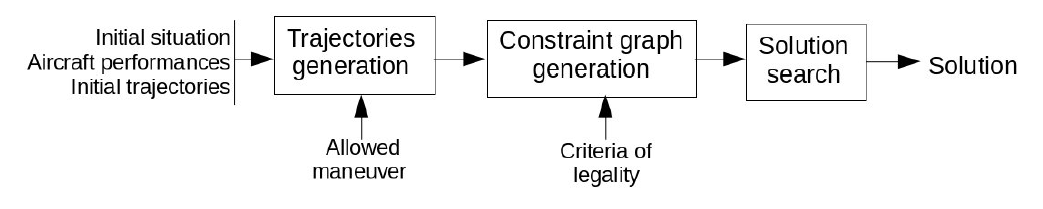
\includegraphics[width=10cm]{images/lumberjack_algo.png}
    \caption{Lumberjack method steps.\cite{chaboud2020tackling}}
\end{figure}

In this model, each aircraft represents a variable of the problem, and the set of its alternative avoidance trajectories constitutes its domain of values.

\begin{figure}[H]
    \centering
    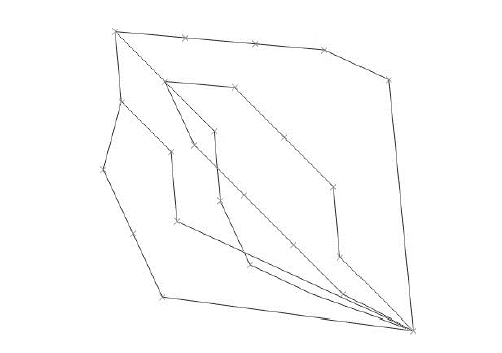
\includegraphics[width=7cm]{images/ex_alternative_fligth.png}
    \caption{Potential trajectories going from upper left to lower right.\cite{chaboud2020tackling}}
\end{figure}

The study compares the performance of the exact solver Toulbar2 with a custom-built ``\ac{SBF}'' algorithm. Analyzing the results highlights a characteristic trait of the \ac{CFN} architecture and Toulbar2. 
The solver handles scaling the number of variables perfectly well. It efficiently resolves conflicts involving a relatively high number of aircraft ($6$ to $8$ planes). 
In contrast, the \ac{SBF} approach collapses under these conditions.

However, Toulbar2's memory saturates quickly when given too many possible trajectories per plane. In other words, it struggles if the domain size becomes too large. This issue can be explained by two factors. 
First is the memory cost of representing constraints in extension. Second is the heavy cost of applying local consistency algorithms to very large domains.

\begin{figure}[H]
    \centering
    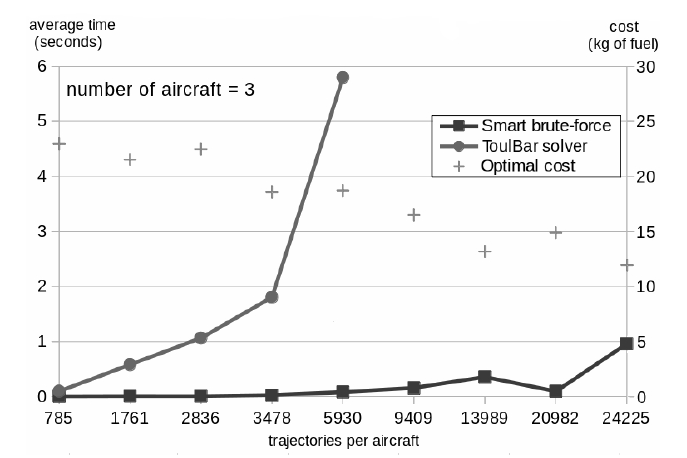
\includegraphics[width=8cm]{images/performance1_SBF_TB2.png}
    \caption{Average solving time over $100$ tests of the \ac{SBF} (squares) and Toulbar2 (circles) approaches
for instances of a Roundabout with $3$ aircraft, function of the number of generated trajectories
per aircraft. Crosses represent the average cost of the optimal solution.\cite{chaboud2020tackling}}
\end{figure}

To overcome these limitations, the authors highlight a pruning method using a "greedy" MinCostMaxClique$^{\ref{algo:mcmc}}$ algorithm. Before launching the exact search, they use a fast, non-optimal greedy heuristic to find an initial valid solution. 
The cost calculated from this solution is then injected into Toulbar2 as an initial ``upper bound''. This trick allows the solver to prune the search tree much faster. 
It removes a considerable number of bad solutions and significantly accelerates the proof of optimality.

\begin{figure}[H]
    \centering
    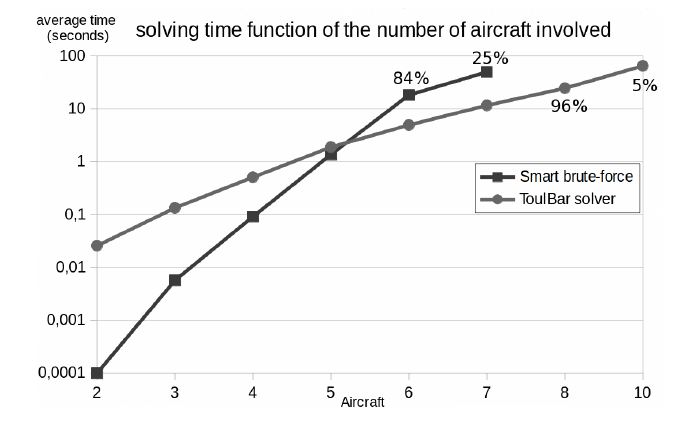
\includegraphics[width=8cm]{images/performance2_SBF_TB2.png}
    \caption{Average solving time over $100$ tests with statistical noise, of \ac{SBF} (squares) and Toulbar2
(circles) approaches for instances of a Roundabout with approx. $850$ trajectories per aircraft,
function of the number of aircraft involved. When a method does not always succeed before the
$60's$ time-out, its success rate is indicated.\cite{chaboud2020tackling}}
\end{figure}

This use case shows that Toulbar2's performance depends heavily on the problem's topology. It also highlights the importance of hybridizing exact methods with fast, non-optimal heuristics. 
This combination guarantees response times that meet real-world industrial requirements.

\subsection{Human resources and global constraints}

Managing space and time is a major challenge. However, human resources planning introduces a different complexity. It requires modeling legal rules and individual preferences.
This subsection highlights how \ac{WCSP} research has had to evolve. It demonstrates the adaptation required to meet the expressivity needed to generate schedules.
\newline

Hospital staff scheduling is an optimization problem known for its high combinatorial complexity. In their study, Métivier et al. (2009)\cite{nurse_rostering_problems} apply the \ac{CFN} formalism and the Toulbar2 solver to generate optimal schedules for nurses. 
They must account for strict staff coverage requirements (hard constraints) as well as staff rest preferences (soft constraints).
\newline

The value of this document for our analysis lies in demonstrating the historical limitations of \acp{WCSP} for this type of problem. Historically, \acp{CFN} were designed around binary constraints. 
However, this type of constraint is poorly suited for modeling human rules. It would require creating an exponentially large constraint network. This makes the solution inefficient.
\newline

To overcome this issue, research around toulbar2 focused on implementing soft global constraints. Unlike a binary constraint, a global constraint simultaneously evaluates a large sequence of assignments. 
For example, it can encompass a nurse's entire week or month in a single evaluation.
Métivier et al. (2009) explain how specific algorithms, based on dynamic programming or flow networks, were integrated directly into Toulbar2. This integration allows the application of local consistencies (such as \ac{EDAC}).
\newline

This article demonstrates a significant evolution. The \ac{WCSP} paradigm is often associated with structural or biological problems. However, it has now achieved a much richer expressivity.
Integrating soft global constraints into toulbar2 proves its true capability. It can now successfully compete with traditional \ac{CP} solvers in the field of human scheduling.

\subsection{Routing and networks}

This final section addresses the allocation of purely abstract and logical resources. The networking and telecommunications field provides an excellent testing ground. It allows us to compare \acp{WCSP} against other major combinatorial optimization standards.
\newline

In their study, Lesaint et al. (2014)\cite{lesaint2014developing} examine a complex problem in telecommunications network allocation and configuration : service subscription conflict management. The issue is as follows. A customer may demand a combination of network services that are technically incompatible due to infrastructure limits. 
When this happens, the provider must find the best compromise. This involves downgrading the service or ignoring certain requested options. The goal is to minimize the overall penalty corresponding to customer dissatisfaction.
This NP-hard decision problem was modeled as a \ac{WCSP}.
\newline

The value of this article lies in its comparative analysis. Instead of isolating Toulbar2, the authors systematically compared the \ac{WCSP} formulation against competing models. These included \ac{MILP} and Partial Weighted Max-SAT. 
The results demonstrate the strength of the \ac{WCSP} approach. By leveraging constraint propagation, it proves highly competitive for dynamically resolving these allocation conflicts.
\newline

This operations research use case provides empirical proof. \ac{WCSP} modeling can compete with historically undisputed paradigms like \ac{MILP} or Max-SAT for allocating abstract resources. 
Toulbar2 can sometimes saturate on certain purely linear problems. However, its modeling flexibility and computational power make it an effective alternative for resolving conflicting query satisfaction problems.

\subsection{Conclusion}

As seen in previous applications, the Toulbar2 solver excels at optimization and planning in deterministic environments. However, resource availability can become uncertain and dynamic. 
A prime example is IoT sensors, whose energy relies on random environmental conditions (Biason et al., 2017)\cite{ieee_transactions_on_mobile_computing}. In these situations, exact planning shows its limitations. 

It then becomes necessary to frame the problem using Markov Decision Processes. Here, Toulbar2 is no longer used as a standalone tool. Instead, it serves as an ``internal computing engine'' powering a probabilistic algorithm.

This need to hybridize exact constraint optimization with models that handle uncertainty marks a natural progression. It directly drives the integration of \acp{WCSP} into the broader fields of Artificial Intelligence and Machine Learning.

\section{Artificial Intelligence \& Machine Learning}


\section{Conclusion}


























% ==================================================================================
% ANNEXES
% ==================================================================================
\newpage
\section{Appendix}
\appendix

\section{Algorithms and Code Snippets} 
\label{annexe:algorithms} % Le label pour faire un renvoi vers la section entière

% --- OPTION 1 : DU PSEUDO-CODE ---
\subsection{Main Heuristic Pseudo-code}

\begin{algorithm}[H]
    \caption{MinCostMaxClique}
    \label{algo:mcmc}
    
    \parbox{\linewidth}{
        \textbf{Where :} \\
        -- $p$, the number of aircraft \\
        -- Vect, a \textit{structure} representing a tuple of trajectories, and composed of an array \textit{tab} of size $p$, containing the id of nodes from the \textit{p}-partite graph ; an \textit{index} ; and a \textit{cost} \\
        -- $H$, a binary min heap of Vect sorted by their \textit{cost}
    }
    
    \vspace{0.3cm}
    \hrule
    \vspace{0.2cm}

    $\text{Vect}\, v; v'$\;
    $v.tab[0 .. p-1] := -1;\, v.index := 0$\;
    $v.tab[v.index]++$\;
    $H.insert(v)$\;
    \While{$H \text{ isn't empty}$}{
        $v := H.\textit{extract\_top}$\;
        \If{$v\, \textit{is legal}$}{
            \If{$v\,\textit{is solution}$}{
                \Return{$v$}\;
            }
            $v' := v$\;
            $v'.\textit{index}++;\, v'.tab[index]++$\;
            $H.insert(v')$\;
            $v.tab[index]++$\;
        }
        $H.insert(v)$\;
    }
    \Return{``No solution''}\;    
\end{algorithm}

\vspace{1cm}

% --- OPTION 2 : DU VRAI CODE (Python, C++, etc.) ---
\subsection{Exemple Python Implementation}

\begin{lstlisting}[language=Python, caption=Python implementation of the heuristic, label=code:python]
def iterative_local_search(S0, I_max):
    best_S = S0
    i = 0
    while i < I_max:
        S_prime = perturbate(best_S)
        S_second = local_search(S_prime)
        
        if cost(S_second) < cost(best_S):
            best_S = S_second
            
        i += 1
    return best_S
\end{lstlisting}

% ==================================================================================================================================
% Biblio

\newpage 
\printbibliography

\end{document}